\chapter{A quick theoretical background}
\label{chap:theoreticalbackground}

In this chapter we introduce briefly some essential terminology for supervised learning. Clearly, a complete mathematical treatment of the field is beyond the scope of this manual, thus we go only briefly over most of the introduced ideas. We refer to any reference textbook for an in-depth treatment.\cite{alpaydin2004introduction,Friedman2009,Mohri2012}

\section{The supervised learning problem}

The starting point in supervised learning is a set $S$, called a \textit{dataset}, composed of $N$ pairs of the form:

\begin{equation}
S = \left\{ x_i, y_i \right\}_{i=1}^N
\label{eq:dataset}
\end{equation}

\noindent where $x \in \mathcal{X}$ and $y \in \mathcal{Y}$. $\mathcal{X}$ and $\mathcal{Y}$ are called the \textit{input} and \textit{output} spaces, respectively.  We call a particular choice of $\mathcal{Y}$ a \textit{task}. Examples of input, tasks and their correspondent data type in Lynx are shown in Table \ref{tab:basicinputs} and \ref{tab:basictasks}. The understanding of data types can be skipped for now, as it will be used more extensively in the later chapters. Although we have currently focused on real-valued input patterns, nothing prevents the toolbox from being extended to more complex situations, such as graphs, sequences, and so on.

\vspace{-2em}

\begin{center}
\begin{table}[t]
{\centering\hfill{}
\begin{tabular}{p{0.3\columnwidth}p{0.5\columnwidth}p{0.2\columnwidth}}
\toprule
Name & Input & Data type \\ 
\midrule
Real-valued vector & $\vect{x} \in \R^{d}$, each element is a \textit{feature} of the pattern & \verb|RealMatrix|  \\
Time-series & $\vect{x} \in \R^n$, each element is the sample of a time-series & \verb|TimeSeries| \\
Kernel vector &  $\vect{x} \in \R^n$, each element is the value of the similarity between two patterns & \verb|KernelMatrix| \\
\bottomrule
\end{tabular}}
\hfill{}
\caption{Summary of inputs defined in the toolbox, and their associated data types.}
\label{tab:basicinputs}
\end{table}
\end{center}

\begin{center}
\begin{table}[t]
{\centering\hfill{}
\begin{tabular}{lll}
\toprule
Name & Input & Output \\ 
\midrule
Regression & $y \in \R$ & \verb|RealVector| \\
Binary classification & $y \in \left\{-1,+1\right\}$ & \verb|BinaryLabelsVector| \\
Multiclass classification & $y \in \left\{1,\dots,M\right\}$ & \verb|IntegerLabelsVector| \\
Multilabel classification & $\vect{y} \in \left\{-1,+1\right\}^M$ & \verb|MultiLabelsMatrix| \\
\bottomrule
\end{tabular}}
\hfill{}
\caption{Summary of tasks defined in the toolbox, and their associated data types.}
\label{tab:basictasks}
\end{table}
\end{center}

We suppose that points in the two spaces are linked by an unknown probabilistic relationship, of which we only know the $N$ samples in $S$. Each sample is also called an \textit{example}, while each element $x \in \mathcal{X}$ is sometimes referred to as a \textit{pattern}.

Informally, the goal of supervised learning is finding a suitable function $f: \mathcal{X} \rightarrow \mathcal{Y}$ such that, given any new sampling $(x, y)$ of the unknown process, the expected error between $f(x)$ and $y$ is minimized. Formally, a \textit{learning algorithm} $\mathcal{A}$ can be defined as a mapping between the space $\mathcal{S}$ of all possible datasets and a given \textit{hypothesis} of the unknown relation:

\begin{equation}
\mathcal{A}(S) : \mathcal{S} \rightarrow \mathcal{H}
\label{eq:learningalgorithm}
\end{equation}

\noindent where $\mathcal{H}$ is called the \textit{hypothesis space}, or \textit{model space}. The notion of error is instead formalized by defining a \textit{loss} function of the form:

\begin{equation}
L(S, f) :  \mathcal{S} \times \mathcal{H} \rightarrow \R
\label{eq:lossfunction}
\end{equation}

\noindent An example of Eq. (\ref{eq:lossfunction}) is the \textit{Mean-Squared Error} (MSE) given by:

\[
L(S, f) = \sum_{(x,y) \in S}(f(x) - y)^2
\]

\noindent In this framework, different learning algorithms differentiate themselves on the choice of the model space, or in the way in which a single hypothesis is extracted from $\mathcal{H}$ given a dataset. It is also possible to compute the performance of an algorithm in term of more complex measures, such as confusion matrices, ROC curves, correlation coefficients, and so on. In this case, we will talk more generally about \textit{performance measures}.

An extension of this basic framework that we have implemented inside Lynx is the \textit{semi-supervised} learning (SSL) framework.\cite{chapelle2006semi} In SSL, we suppose having available an additional unlabeled dataset of $M$ input patterns $U = \left\{ x_i \right\}_{i=1}^M$. An SSL algorithm uses this additional information trying to improve its own accuracy. Formally, if we denote by $\mathcal{U}$ the space of all possible unlabeled datasets, an SSL algorithm $\mathcal{A}_{\mbox{\scriptsize SSL}}$ is a mapping of the form:

\begin{equation}
\mathcal{A}_{\mbox{\scriptsize SSL}}(S,U): \mathcal{S} \times \mathcal{U} \rightarrow \mathcal{H}
\label{eq:ssl}
\end{equation}

\noindent where the difference with Eq. \eqref{eq:learningalgorithm} is the presence of the additional input $U$.

\section{Some additional terminology}

We call an \textit{experiment} the test of a particular learning algorithm on a dataset. For a realistic workflow, refer to Fig. \ref{fig:workflow}. The dataset, before being used, is processed by one (or more) \textit{preprocessors}. A typical example of preprocessor is the \textit{Principal Component Analysis} (PCA). The dataset is not used all for training, but it is partitioned in a \textit{training set} and a \textit{testing set}. The way in which data is subdivided is called a \textit{partitioning strategy}. A partitioning strategy can also define multiple splits for a single dataset (e.g., k-fold cross-validation procedures): in this case, each split is called a \textit{fold}. Finally, in Fig. \ref{fig:workflow} the learning algorithm is encapsulated inside a generic ``\textit{wrapper}'' object, that we define to be any method performing some additional optimization over the training procedure or the resulting model. This rather general definition includes techniques for optimizing the parameters of the algorithm, selecting a suitable subset of features, or training an ensemble of classifiers \cite{alpaydin2004introduction}.

\begin{figure}[t]
\centering
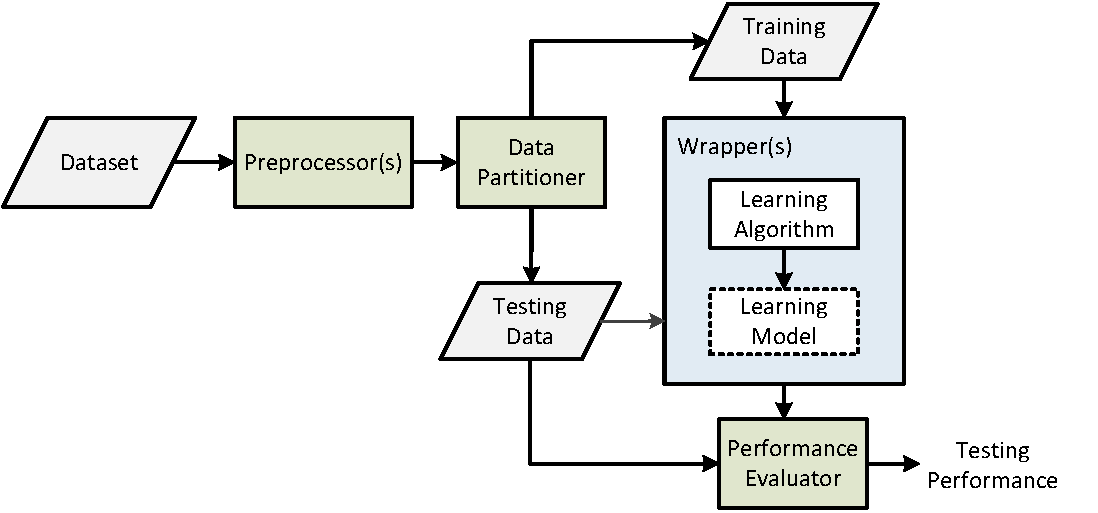
\includegraphics[scale=0.6]{./images/Disegno3}
\caption{Workflow of a single experiment}
\label{fig:workflow}
\end{figure}